\documentclass[english,10pt,a4paper]{article}
\usepackage{tcolorbox}
\usepackage{ulem} %math
\usepackage{amsmath}
\usepackage{amsfonts}
\usepackage{amssymb}
\usepackage{graphicx}
\usepackage{enumerate}


%Create a box for theorems
%\begin{theo}[titel] %optional
%tekst
%\end{theo}
\newenvironment{theo}[1][Vigtigt]{%
\begin{tcolorbox}[colback=green!5,colframe=green!40!black,title=\textbf{#1}]
}{%
\end{tcolorbox}
}




%Create a square matrix
%\begin{ArgMat}{2}
%21 & 22 & 23 \\  
%a & b & c
%\end{ArgMat}
%
% Info: http://tex.stackexchange.com/questions/2233/whats-the-best-way-make-an-augmented-coefficient-matrix
%
\newenvironment{ArgMat}{%
$
  \left[\begin{array}{@{}*{100}{r}r@{}}
}{%
  \end{array}\right]
  $
}

\newenvironment{deter}{%
$
  \left|\begin{array}{@{}*{100}{r}r@{}}
}{%
  \end{array}\right|
  $
}


%Create multiple lines with holes
%\begin{SysEqu}
%x_1 && &- &5x_3 &+ &2x_4=& 1 \\
%x_1 &+ &x_2 &+ &x_3 && =& 4 \\
%&&&&&&0 =& 0
%\end{SysEqu}
\newenvironment{SysEqu}{%
$  \setlength\arraycolsep{0.1em}
  \begin{array}{@{}*{100}{r}r@{}}
}{%
  \end{array}$
}

%Create solution for x_1, x_n...
%\begin{solu}
%x_1 &= d \\
%x_2 &= e \\
%x_3 &= s
%\end{solu}
\newenvironment{solu}{%
$
  \setlength\arraycolsep{0.1em}
  \left\{\begin{array}{@{}*{100}{r}r@{}}
}{%
  \end{array}\right.
$
}

\usepackage{lastpage}


\newcommand{\HRule}{\rule{\linewidth}{0.8mm}}

%Tekst i fotter
\newcommand{\footerText}{\thepage\xspace /\pageref{LastPage}}
\newcommand{\ProjectName}{433 MHz styring af AeroQuad}


\chapterstyle{hangnum}




\nouppercaseheads
\makepagestyle{mystyle} 

\makeevenhead{mystyle}{}{\\ \leftmark}{} 
\makeoddhead{mystyle}{}{\\ \leftmark}{} 
\makeevenfoot{mystyle}{}{\footerText}{} 
\makeoddfoot{mystyle}{}{\footerText}{} 
\makeatletter
\makepsmarks{mystyle}{% Overskriften på sidehovedet
  \createmark{chapter}{left}{shownumber}{\@chapapp\ }{.\ }} 
\makeatother
\makefootrule{mystyle}{\textwidth}{\normalrulethickness}{0.4pt}
\makeheadrule{mystyle}{\textwidth}{\normalrulethickness}

\makepagestyle{plain}
\makeevenhead{plain}{}{}{}
\makeoddhead{plain}{}{}{}
\makeevenfoot{plain}{}{\footerText}{}
\makeoddfoot{plain}{}{\footerText}{}
\makefootrule{plain}{\textwidth}{\normalrulethickness}{0.4pt}

\pagestyle{mystyle}

%%----------------------------------------------------------------------
%
%%Redefining chapter style
%%\renewcommand\chapterheadstart{\vspace*{\beforechapskip}}
%\renewcommand\chapterheadstart{\vspace*{10pt}}
%\renewcommand\printchaptername{\chapnamefont }%\@chapapp}
%\renewcommand\chapternamenum{\space}
%\renewcommand\printchapternum{\chapnumfont \thechapter}
%\renewcommand\afterchapternum{\space: }%\par\nobreak\vskip \midchapskip}
%\renewcommand\printchapternonum{}
%\renewcommand\printchaptertitle[1]{\chaptitlefont #1}
\setlength{\beforechapskip}{0pt} 
\setlength{\afterchapskip}{0pt} 
%\setlength{\voffset}{0pt} 
\setlength{\headsep}{25pt}
%\setlength{\topmargin}{35pt}
%%\setlength{\headheight}{102pt}
%\setlength{\textheight}{302pt}
\renewcommand\afterchaptertitle{\par\nobreak\vskip \afterchapskip}
%%----------------------------------------------------------------------




%Sidehoved og -fod pakke
%Margin
\usepackage[left=2cm,right=2cm,top=2.5cm,bottom=2cm]{geometry}
\usepackage{lastpage}



%%URL kommandoer og sidetal farve
%%Kaldes med \url{www...}
%\usepackage{color} %Skal også bruges
\usepackage{hyperref}
\hypersetup{ 
	colorlinks	= true, 	% false: boxed links; true: colored links
    urlcolor	= blue,		% color of external links
    linkcolor	= black, 	% color of page numbers
    citecolor	= blue,
}



%Mellemrum mellem linjerne    
\linespread{1.5}


%Seperated files
%--------------------------------------------------
%Opret filer således:
%\documentclass[Navn-på-hovedfil]{subfiles}
%\begin{document}
% Indmad
%\end{document}
%
% I hovedfil inkluderes således:
% \subfile{navn-på-subfil}
%--------------------------------------------------
\usepackage{subfiles}

%Prevent wierd placement of figures
%\usepackage[section]{placeins}

%Standard sti at søge efter billeder
%--------------------------------------------------
%\begin{figure}[hbtp]
%\centering
%\includegraphics[scale=1]{filnavn-for-png}
%\caption{Titel}
%\label{fig:referenceNavn}
%\end{figure}
%--------------------------------------------------
\usepackage{graphicx}
\usepackage{subcaption}
\usepackage{float}
\graphicspath{{../Figures/}}

%Speciel skrift for enkelt linje kode
%--------------------------------------------------
%Udskriver med fonten 'Courier'
%Mere info her: http://tex.stackexchange.com/questions/25249/how-do-i-use-a-particular-font-for-a-small-section-of-text-in-my-document
%Eksempel: Funktionen \code{void Hello()} giver et output
%--------------------------------------------------
\newcommand{\code}[1]{{\fontfamily{pcr}\selectfont #1}}


% Følgende er til koder.
%----------------------------------------------------------
%\begin{lstlisting}[caption=Overskrift på boks, style=Code-C++, label=lst:referenceLabel]
%public void hello(){}
%\end{lstlisting}
%----------------------------------------------------------

%Exstra space
\usepackage{xspace}
%Navn på bokse efterfulgt af \xspace (hvis det skal være mellemrum
%gives det med denne udvidelse. Ellers ingen mellemrum.
\newcommand{\codeTitle}{Kodeudsnit\xspace}

%Pakker der skal bruges til lstlisting
\usepackage{listings}
\usepackage{color}
\usepackage{textcomp}
\definecolor{listinggray}{gray}{0.9}
\definecolor{lbcolor}{rgb}{0.9,0.9,0.9}
\renewcommand{\lstlistingname}{\codeTitle}
\lstdefinestyle{Code}
{
	keywordstyle	= \bfseries\ttfamily\color[rgb]{0,0,1},
	identifierstyle	= \ttfamily,
	commentstyle	= \color[rgb]{0.133,0.545,0.133},
	stringstyle		= \ttfamily\color[rgb]{0.627,0.126,0.941},
	showstringspaces= false,
	basicstyle		= \small,
	numberstyle		= \footnotesize,
%	numbers			= left, % Tal? Udkommenter hvis ikke
	stepnumber		= 2,
	numbersep		= 6pt,
	tabsize			= 2,
	breaklines		= true,
	prebreak 		= \raisebox{0ex}[0ex][0ex]{\ensuremath{\hookleftarrow}},
	breakatwhitespace= false,
%	aboveskip		= {1.5\baselineskip},
  	columns			= fixed,
  	upquote			= true,
  	extendedchars	= true,
 	backgroundcolor = \color{lbcolor},
	lineskip		= 1pt,
%	xleftmargin		= 17pt,
%	framexleftmargin= 17pt,
	framexrightmargin	= 0pt, %6pt
%	framexbottommargin	= 4pt,
}

%Bredde der bruges til indryk
%Den skal være 6 pt mindre
\usepackage{calc}
\newlength{\mywidth}
\setlength{\mywidth}{\textwidth-6pt}


% Forskellige styles for forskellige kodetyper
\usepackage{caption}
\DeclareCaptionFont{white}{\color{white}}
\DeclareCaptionFormat{listing}%
{\colorbox[cmyk]{0.43, 0.35, 0.35,0.35}{\parbox{\mywidth}{\hspace{5pt}#1#2#3}}}
\captionsetup[lstlisting]
{
	format			= listing,
	labelfont		= white,
	textfont		= white, 
	singlelinecheck	= false, 
	width			= \mywidth,
	margin			= 0pt, 
	font			= {bf,footnotesize}
}

\lstdefinestyle{Code-C} {language=C, style=Code}
\lstdefinestyle{Code-Java} {language=Java, style=Code}
\lstdefinestyle{Code-C++} {language=[Visual]C++, style=Code}
\lstdefinestyle{Code-VHDL} {language=VHDL, style=Code}
\lstdefinestyle{Code-Bash} {language=Bash, style=Code}

%Text typesetting
%--------------------------------------------------------
%\usepackage{baskervald}
\usepackage{lmodern}
\usepackage[T1]{fontenc}              
\usepackage[utf8]{inputenc}         
\usepackage[english]{babel}       

\setlength{\parindent}{0pt}
\nonzeroparskip

%\setaftersubsecskip{1sp}
%\setaftersubsubsecskip{1sp}
 


%Dybde på indholdsfortegnelse
%----------------------------------------------------------
%Chapter, section, subsection, subsubsection
%----------------------------------------------------------
\setcounter{secnumdepth}{3}
\setcounter{tocdepth}{3}


%Tables
%----------------------------------------------------------
\usepackage{tabularx}
\usepackage{array}
\usepackage{multirow} 
\usepackage{multicol} 
\usepackage{booktabs}
\usepackage{wrapfig}
\renewcommand{\arraystretch}{1.5}



%Misc
%----------------------------------------------------------
\usepackage{cite}
\usepackage{appendix}
\usepackage{amssymb}
\usepackage{url,ragged2e}
\usepackage{enumerate}
\usepackage{amsmath} %Math bibliotek


\usepackage{longtable}


\title{Workshop 1}
\begin{document}
\maketitle

\section*{Problem 1}
$\bigg(p \wedge \Big( q \Rightarrow (\sim r)\Big) \bigg)  \Rightarrow  \Big( (\sim q) \vee r \Big)$:

\begin{table}[h]
\centering
	\begin{tabular}{c|c|c|c|c|c}
	\textbf{p} & \textbf{q} & \textbf{r} & \textbf{$\bigg(p \wedge \Big( q \Rightarrow (\sim r)\Big) \bigg)$} & \textbf{$\Big( (\sim q) \vee r \Big)$} &\textbf{$\bigg(p \wedge \Big( q \Rightarrow (\sim r)\Big) \bigg)  \Rightarrow  \Big( (\sim q) \vee r \Big)$}\\\hline
	F & F & F & F & T & T\\	\hline
	F & F & T & F & F & T\\	\hline
	F & T & F & F & T & T\\	\hline
	F & T & T & F & T & T\\	\hline
	T & F & F & T & T & T\\	\hline
	T & F & T & T & T & T\\	\hline
	T & T & F & F & F & F\\	\hline
	T & T & T & T & T & T\\	\hline
	\end{tabular}
\caption{Truthtable}
\end{table}

\section*{Problem 2}


\begin{enumerate}[a]
\item $\Big( p \wedge (\sim q)\Big) \wedge \Big(( \sim p) \vee q\Big) $.
\begin{table}[h]
\centering
	\begin{tabular}{c|c|c|c|c}
	\textbf{p} & \textbf{q} & \textbf{$\Big( p \wedge (\sim q)\Big)$} & \textbf{$ \Big(( \sim p) \vee q\Big) $}  & $\Big( p \wedge (\sim q)\Big) \wedge \Big(( \sim p) \vee q\Big) $\\\hline
	T & T & F & T & F\\ 	\hline
	T & F & T & F & F\\ 	\hline 
	F & T & F & T & F\\ 	\hline 
	F & F & F & T & F\\ 	\hline 
	\end{tabular}
\caption{Truthtable}
\label{tab:title}
\end{table}
From the last column it is detminated that it is a contradiction.

\item $(p \Rightarrow q) \Rightarrow (p \vee q)$. From the last column it is detminated to be neither.
\begin{table}[h]
\centering
	\begin{tabular}{c|c|c|c|c}
	\textbf{p} & \textbf{q} & $(p \Rightarrow q)$ & $(p \vee q)$ & $(p \Rightarrow q) \Rightarrow (p \vee q)$\\\hline
	T & T & T & T & T\\ 	\hline
	T & F & F & T & T\\ 	\hline 
	F & T & T & T & T\\ 	\hline 
	F & F & T & F & F\\ 	\hline 
	\end{tabular}
\caption{Truthtable}
\label{tab:title}
\end{table}

\end{enumerate}

\newpage
\section*{Problem 3}

\begin{enumerate}[a]
\item For $p \wedge p \equiv p$:
\begin{table}[h]
\centering
	\begin{tabular}{c|c|c}
	\textbf{p} & $p \wedge p$ &\textbf{$p \wedge p \equiv p$} \\\hline
	T & T  & T\\\hline 
	F & F & T
	\end{tabular}
\caption{Truthtable}
\label{tab:title}
\end{table}

\item  For $p \vee (p \wedge q) \equiv p$ and $p \wedge (p \vee q) \equiv p$:
\begin{table}[h]
\centering
	\begin{tabular}{c|c|c|c|c|c}
	\textbf{p} & 
	\textbf{q} & 
	$p \wedge q$ & 
	$p \vee q$ & 
	$p \vee (p \wedge q) \equiv p$ & 
	$p \wedge (p \vee q) \equiv p$ \\\hline
	T & T & T & T & T & T\\\hline 
	T & F & F & T & T & T\\\hline
	F & T & F & T & F & F\\\hline
	F & F & F & F & F & F\\\hline
	\end{tabular}
\caption{Truthtable}
\label{tab:title}
\end{table}

\item For $p \wedge T \equiv p$ and $p \vee T \equiv T$:
\begin{table}[h]
\centering
	\begin{tabular}{c|c|c|c}
	\textbf{p} & 
	\textbf{T} & 
	$p \wedge T \equiv p$ & 
	$p \vee T \equiv T$   \\\hline
	T & T & T & T \\\hline 
	F & T & F & T \\\hline
	\end{tabular}
\caption{Truthtable}
\label{tab:title}
\end{table}


\item For $p \wedge F \equiv F$ and $p \vee F \equiv p$:
\begin{table}[h]
\centering
	\begin{tabular}{c|c|c|c}
	\textbf{p} & 
	\textbf{F} & 
	$p \wedge F \equiv F$ & 
	$p \vee F \equiv p$   \\\hline
	T & F & F & T \\\hline 
	F & F & F & F \\\hline
	\end{tabular}
\caption{Truthtable}
\label{tab:title}
\end{table}
\end{enumerate}



\section*{Problem 4}
This is most likely because, the computer must do the operation which takes time (not much but some) and to save time the computer "short circuit".


\section*{Problem 5}
An example could be \code{if(2 == 3 || false == false)\{...\}} -- which shows the first condition will cause the \code{if} to break.



\newpage
\section*{Problem 7}
\begin{figure}[hbtp]
\centering
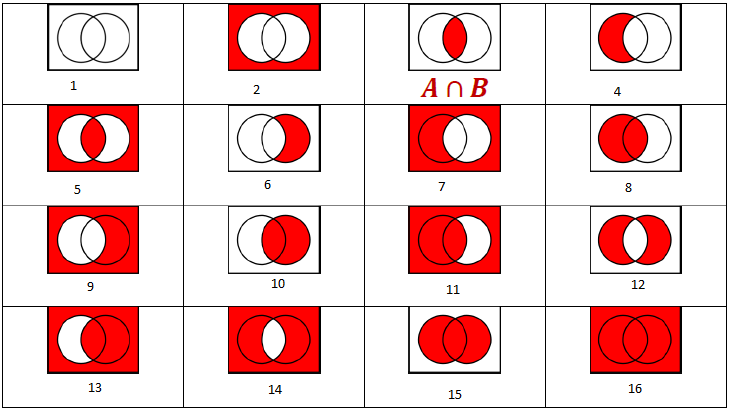
\includegraphics[scale=0.75]{p7}
\caption{Venn diagrammer}
\label{fig:venn}
\end{figure}
On Figure \ref{fig:venn} the Venn diagrams have been numbered.
The following show the correct logic:
\begin{enumerate}
\item $\emptyset$
\item $\neg A \vee \neg B$
\item $A \cap B$
\item $\neg B \cap A$
\item $(A \cap B) \cup ( \neg A \vee \neg B)$
\item $\neg A \cap B$
\item $\neg B$
\item A
\item $\neg A$
\item B
\item $A \cup \neg B$
\item $(A \cup B) \cup \neg (A \cap B)$
\item $B \cup r$
\item $r \cup \neg(A\cap B)$
\item $A\cup B $
\item $\neg \emptyset$
\end{enumerate}


\newpage
\section*{Problem 8}



\end{document}